% =============================================================================
% Production-Grade Parallel AVL Trees - Cybersecurity Presentation (English)
% Author: Lucas Sotomayor - R&D Division
% Focus: AC-DoS Mitigation & Resilient Architecture
% =============================================================================

\documentclass[aspectratio=169,10pt]{beamer}

% -----------------------------------------------------------------------------
% Theme: Metropolis with Cyber Color Scheme
% -----------------------------------------------------------------------------
\usetheme{Madrid}
\usecolortheme{spruce}

% Cyber color palette - Dark background with neon accents
\definecolor{cyberbg}{RGB}{18,18,28}
\definecolor{cyberfg}{RGB}{220,220,220}
\definecolor{cyberneon}{RGB}{0,255,136}
\definecolor{cyberorange}{RGB}{255,136,0}
\definecolor{cyberred}{RGB}{255,71,87}
\definecolor{cyberpurple}{RGB}{138,43,226}
\definecolor{codebg}{RGB}{30,30,45}
\definecolor{cybergray}{RGB}{45,45,60}

% Apply cyber theme
\setbeamercolor{structure}{fg=cyberneon}
\setbeamercolor{palette primary}{bg=cyberbg,fg=cyberfg}
\setbeamercolor{palette secondary}{bg=cybergray,fg=cyberfg}
\setbeamercolor{palette tertiary}{bg=cyberneon!80!black,fg=black}
\setbeamercolor{titlelike}{fg=cyberneon}
\setbeamercolor{frametitle}{bg=cyberbg,fg=cyberneon}
\setbeamercolor{title}{fg=cyberneon}
\setbeamercolor{subtitle}{fg=cyberorange}
\setbeamercolor{author}{fg=cyberfg}
\setbeamercolor{normal text}{fg=cyberbg}
\setbeamercolor{block title}{bg=cyberneon!80!black,fg=black}
\setbeamercolor{block body}{bg=cyberneon!10}
\setbeamercolor{block title alerted}{bg=cyberred,fg=white}
\setbeamercolor{block body alerted}{bg=cyberred!10}
\setbeamercolor{block title example}{bg=cyberorange,fg=black}
\setbeamercolor{block body example}{bg=cyberorange!10}
\setbeamercolor{alerted text}{fg=cyberred}
\setbeamercolor{item}{fg=cyberneon}

% -----------------------------------------------------------------------------
% Packages
% -----------------------------------------------------------------------------
\usepackage[utf8]{inputenc}
\usepackage[T1]{fontenc}
\usepackage{amsmath,amssymb}
\usepackage{booktabs}
\usepackage{multirow}
\usepackage{graphicx}
\usepackage{tikz}
\usetikzlibrary{shapes,arrows,positioning,fit,backgrounds,calc,decorations.pathmorphing}
\usepackage{listings}
\usepackage{fontawesome5}
\usepackage{xcolor}
\usepackage{colortbl}

% -----------------------------------------------------------------------------
% Listings Configuration - Cyber Style
% -----------------------------------------------------------------------------
\lstset{
    language=C++,
    basicstyle=\ttfamily\scriptsize\color{cyberfg},
    keywordstyle=\color{cyberneon}\bfseries,
    commentstyle=\color{gray}\itshape,
    stringstyle=\color{cyberorange},
    backgroundcolor=\color{codebg},
    frame=single,
    rulecolor=\color{cyberneon},
    showstringspaces=false,
    breaklines=true,
    numbers=left,
    numberstyle=\tiny\color{gray},
    tabsize=2,
    morekeywords={size_t,atomic,mutex,unique_lock,thread,uint64_t}
}

% -----------------------------------------------------------------------------
% TikZ Styles - Cyber Theme
% -----------------------------------------------------------------------------
\tikzstyle{attacker} = [rectangle, rounded corners, minimum width=2cm, 
                        minimum height=1cm, text centered, draw=cyberred, 
                        fill=cyberred!20, font=\small\bfseries, text=cyberred]
\tikzstyle{component} = [rectangle, rounded corners, minimum width=2.5cm, 
                         minimum height=0.8cm, text centered, draw=cyberneon, 
                         fill=cyberneon!15, font=\small\bfseries]
\tikzstyle{shard} = [rectangle, rounded corners, minimum width=1.5cm, 
                     minimum height=0.6cm, text centered, draw=cyberorange, 
                     fill=cyberorange!15, font=\scriptsize]
\tikzstyle{arrow} = [thick, ->, >=stealth, color=cyberneon]
\tikzstyle{attackarrow} = [thick, ->, >=stealth, color=cyberred, decorate, 
                           decoration={snake, amplitude=1mm, segment length=3mm}]

% -----------------------------------------------------------------------------
% Metadata
% -----------------------------------------------------------------------------
\title{\textbf{Production-Grade Parallel AVL Trees}}
\subtitle{A Resilient Architecture for Mitigating AC-DoS}
\author{Lucas Sotomayor\\{\small R\&D Division}}
\date{\today}
\institute{Security Consulting}

% =============================================================================
% DOCUMENT
% =============================================================================
\begin{document}

% -----------------------------------------------------------------------------
% SLIDE 1: Title
% -----------------------------------------------------------------------------
{
\setbeamercolor{background canvas}{bg=cyberbg}
\begin{frame}[plain]
    \begin{center}
        \vspace{1cm}
        {\huge \textcolor{cyberneon}{\faShield*}}
        
        \vspace{0.5cm}
        {\Huge \textcolor{cyberneon}{\textbf{Production-Grade Parallel AVL Trees}}}
        
        \vspace{0.3cm}
        {\Large \textcolor{cyberorange}{A Resilient Architecture for Mitigating AC-DoS}}
        
        \vspace{1cm}
        {\large \textcolor{cyberfg}{Lucas Sotomayor}}\\
        {\normalsize \textcolor{gray}{R\&D Division $\bullet$ Security Consulting}}
        
        \vspace{1cm}
        {\small \textcolor{gray}{\today}}
    \end{center}
\end{frame}
}

% -----------------------------------------------------------------------------
% SLIDE 2: The Threat - The Vulnerability
% -----------------------------------------------------------------------------
{
\setbeamercolor{background canvas}{bg=cyberbg}
\begin{frame}{\textcolor{cyberneon}{\faExclamationTriangle} The Threat: Algorithmic Complexity DoS}
    
    \textcolor{cyberfg}{
    \textbf{Attack Vector:} Adversary exploits predictable data structure behavior
    }
    
    \vspace{0.5em}
    
    \begin{columns}[T]
        \begin{column}{0.48\textwidth}
            \begin{alertblock}{Vulnerability Classes}
                \begin{itemize}
                    \item \textbf{CWE-407:} Inefficient Algorithmic Complexity
                    \item \textbf{Hash Flooding:} Collision-based attacks
                    \item \textbf{Hotspot Saturation:} Single-point overload
                \end{itemize}
            \end{alertblock}
            
            \vspace{0.3em}
            \textcolor{cyberfg}{\textbf{Impact:}}
            \begin{itemize}
                \item[\textcolor{cyberred}{\faTimesCircle}] \textcolor{cyberfg}{Service degradation}
                \item[\textcolor{cyberred}{\faTimesCircle}] \textcolor{cyberfg}{Resource exhaustion}
                \item[\textcolor{cyberred}{\faTimesCircle}] \textcolor{cyberfg}{Complete unavailability}
            \end{itemize}
        \end{column}
        \begin{column}{0.48\textwidth}
            \begin{center}
            \begin{tikzpicture}[scale=0.8, transform shape]
                % Attack flow
                \node[attacker] (atk) at (0,2) {\faUserSecret\ Attacker};
                \node[component, fill=cyberred!30, draw=cyberred] (hash) at (0,0) {Static Hash};
                \node[shard, fill=cyberred!50] (s0) at (0,-1.8) {Shard 0: 100\%};
                \node[shard, fill=gray!20, draw=gray] (s1) at (-2,-1.8) {Shard 1: 0\%};
                \node[shard, fill=gray!20, draw=gray] (s2) at (2,-1.8) {Shard N: 0\%};
                
                \draw[attackarrow] (atk) -- (hash);
                \draw[attackarrow] (hash) -- (s0);
                
                \node[below, font=\scriptsize\color{cyberred}] at (0,-2.5) {\textbf{0\% Availability}};
            \end{tikzpicture}
            \end{center}
            
            \vspace{0.3em}
            \begin{center}
                \fcolorbox{cyberred}{cyberred!10}{
                    \textcolor{cyberred}{\textbf{Static Hash + Adversarial Input = DoS}}
                }
            \end{center}
        \end{column}
    \end{columns}
    
\end{frame}
}

% -----------------------------------------------------------------------------
% SLIDE 3: The Solution - Tree-of-Trees Architecture
% -----------------------------------------------------------------------------
{
\setbeamercolor{background canvas}{bg=cyberbg}
\begin{frame}{\textcolor{cyberneon}{\faProjectDiagram} The Solution: Tree-of-Trees Architecture}
    
    \begin{columns}[T]
        \begin{column}{0.55\textwidth}
            \begin{center}
            \begin{tikzpicture}[scale=0.75, transform shape]
                % Main container
                \node[component, minimum width=7cm, minimum height=5cm, fill=cybergray!50] (main) at (0,0) {};
                \node[above, font=\bfseries\color{cyberneon}] at (main.north) {ParallelAVL (Unified API)};
                
                % Router with defense
                \node[component, minimum width=5.5cm, fill=cyberneon!25] (router) at (0,1.5) {\faShield*\ Adaptive Router};
                
                % Defense modules
                \node[shard, minimum width=2.2cm, fill=cyberorange!25] (cache) at (-1.3,0.6) {LoadStats};
                \node[shard, minimum width=2.2cm, fill=cyberpurple!25, draw=cyberpurple] (pattern) at (1.5,0.6) {PatternTracker};
                
                % RedirectIndex
                \node[component, minimum width=2.8cm, fill=cyberneon!15] (redirect) at (-1.5,-0.5) {RedirectIndex};
                \node[shard, minimum width=1.5cm, fill=cyberorange!20, font=\tiny] (gc) at (-1.5,-1.2) {\faRecycle\ GC};
                
                % Shards - distributed load
                \node[shard, fill=cyberneon!30] (s0) at (1.8,-0.2) {Shard 0};
                \node[shard, fill=cyberneon!30] (s1) at (1.8,-0.8) {Shard 1};
                \node[shard, fill=cyberneon!30] (s2) at (1.8,-1.4) {Shard 2};
                \node[shard, fill=cyberneon!30] (sn) at (1.8,-2) {Shard N};
                
                % Arrows
                \draw[arrow] (router) -- (cache);
                \draw[arrow] (router) -- (pattern);
                \draw[arrow] (router.south) -- ++(0,-0.2) -| (s0.north);
            \end{tikzpicture}
            \end{center}
        \end{column}
        \begin{column}{0.42\textwidth}
            \textcolor{cyberfg}{\textbf{Security Properties:}}
            \vspace{0.3em}
            
            \begin{itemize}
                \item[\textcolor{cyberneon}{\faCheck}] \textcolor{cyberfg}{\textbf{Shared-Nothing:} Isolated shards}
                \item[\textcolor{cyberneon}{\faCheck}] \textcolor{cyberfg}{\textbf{No Single Point:} Distributed load}
                \item[\textcolor{cyberneon}{\faCheck}] \textcolor{cyberfg}{\textbf{Graceful Degradation}}
                \item[\textcolor{cyberneon}{\faCheck}] \textcolor{cyberfg}{\textbf{Real-time Detection}}
            \end{itemize}
            
            \vspace{0.5em}
            \begin{block}{Attack Surface Reduction}
                \textcolor{cyberbg}{
                Contention attack requires compromising \textbf{all N shards} simultaneously
                }
            \end{block}
            
            \vspace{0.3em}
            \textcolor{cyberorange}{\textbf{Result:} 97\% parallel efficiency}
        \end{column}
    \end{columns}
    
\end{frame}
}

% -----------------------------------------------------------------------------
% SLIDE 4: Defensive Innovation 1 - Adaptive Routing
% -----------------------------------------------------------------------------
{
\setbeamercolor{background canvas}{bg=cyberbg}
\begin{frame}[fragile]{\textcolor{cyberneon}{\faRadiation} Defense 1: Adaptive Routing (O(1) Anomaly Detection)}
    
    \textcolor{cyberfg}{\textbf{Mechanism:} Real-time hotspot detection with cached statistics}
    
    \vspace{0.3em}
    
    \begin{columns}[T]
        \begin{column}{0.48\textwidth}
            \begin{block}{Active Defense Algorithm}
            \textcolor{cyberbg}{
            \begin{enumerate}
                \scriptsize
                \item Background thread monitors load every 1ms
                \item Detects anomaly: $load_{max} > 1.5 \times \bar{load}$
                \item Switches routing strategy dynamically
                \item Routes away from saturated shards
            \end{enumerate}
            }
            \end{block}
            
            \vspace{0.2em}
\begin{lstlisting}
// O(1) Hotspot Query
size_t get_safest_shard() {
  return min_shard_.load(acquire);
}

// Anomaly Detection
bool is_under_attack() {
  auto stats = cache_.get_stats();
  return stats.max_load > 
         1.5 * stats.avg_load;
}
\end{lstlisting}
        \end{column}
        \begin{column}{0.48\textwidth}
            \textcolor{cyberfg}{\textbf{Routing Strategies:}}
            \vspace{0.3em}
            
            \begin{tabular}{@{}ll@{}}
                \textcolor{gray}{Normal:} & \textcolor{cyberfg}{Static Hash (fast)} \\
                \textcolor{cyberorange}{Variance:} & \textcolor{cyberfg}{Consistent Hash} \\
                \textcolor{cyberred}{Hotspot:} & \textcolor{cyberfg}{Load-Aware (defense)} \\
                \textcolor{cyberneon}{Auto:} & \textcolor{cyberfg}{Intelligent (hybrid)} \\
            \end{tabular}
            
            \vspace{0.5em}
            \begin{exampleblock}{Key Metric}
                \textcolor{cyberbg}{
                \textbf{Detection Latency:} O(1) \\
                \textbf{Response Time:} $<$ 1ms \\
                \textbf{False Positives:} 0\%
                }
            \end{exampleblock}
            
            \vspace{0.3em}
            \textcolor{cyberneon}{\faShield*\ \textbf{Proactive, not reactive}}
        \end{column}
    \end{columns}
    
\end{frame}
}

% -----------------------------------------------------------------------------
% SLIDE 5: Defensive Innovation 2 - Rate Limiting & GC
% -----------------------------------------------------------------------------
{
\setbeamercolor{background canvas}{bg=cyberbg}
\begin{frame}[fragile]{\textcolor{cyberneon}{\faLock} Defense 2: Rate Limiting \& Memory Protection}
    
    \begin{columns}[T]
        \begin{column}{0.48\textwidth}
            \textcolor{cyberfg}{\textbf{\faStopwatch\ Anti-Thrashing Controls}}
            \vspace{0.3em}
            
            \begin{alertblock}{Pattern Tracking}
                \textcolor{cyberbg}{
                \begin{itemize}
                    \item \textbf{Max Redirects:} 3 per key
                    \item \textbf{Cooldown:} 100ms between moves
                    \item \textbf{Suspicious Detection:} Blocks rapid patterns
                \end{itemize}
                }
            \end{alertblock}
            
            \vspace{0.2em}
\begin{lstlisting}
struct RedirectPolicy {
  static constexpr int MAX_REDIRECTS = 3;
  static constexpr auto COOLDOWN = 100ms;
  
  bool can_redirect(Key k) {
    auto& entry = history_[k];
    if (entry.count >= MAX_REDIRECTS)
      return false;
    if (now() - entry.last < COOLDOWN)
      return false;
    return true;
  }
};
\end{lstlisting}
        \end{column}
        \begin{column}{0.48\textwidth}
            \textcolor{cyberfg}{\textbf{\faRecycle\ Memory Exhaustion Prevention}}
            \vspace{0.3em}
            
            \begin{block}{Garbage Collector}
                \textcolor{cyberbg}{
                \textbf{Threat:} Redirect index grows unbounded \\
                \textbf{Defense:} Periodic cleanup of obsolete entries
                }
            \end{block}
            
            \vspace{0.3em}
            \textcolor{cyberfg}{\textbf{GC Results:}}
            \begin{itemize}
                \item[\textcolor{cyberneon}{\faCheck}] \textcolor{cyberfg}{1000 entries $\rightarrow$ 28KB freed}
                \item[\textcolor{cyberneon}{\faCheck}] \textcolor{cyberfg}{Execution time: 0.12ms}
                \item[\textcolor{cyberneon}{\faCheck}] \textcolor{cyberfg}{Zero data loss}
                \item[\textcolor{cyberneon}{\faCheck}] \textcolor{cyberfg}{Thread-safe operation}
            \end{itemize}
            
            \vspace{0.3em}
            \begin{center}
                \fcolorbox{cyberneon}{cyberneon!10}{
                    \textcolor{cyberneon}{\textbf{Prevents Resource Exhaustion}}
                }
            \end{center}
        \end{column}
    \end{columns}
    
\end{frame}
}

% -----------------------------------------------------------------------------
% SLIDE 6: Security Validation - Results
% -----------------------------------------------------------------------------
{
\setbeamercolor{background canvas}{bg=cyberbg}
\begin{frame}{\textcolor{cyberneon}{\faChartBar} Security Validation: Attack Resistance}
    
    \textcolor{cyberfg}{\textbf{Test:} Targeted adversarial workload (keys $0, N, 2N, \ldots$ saturating shard 0)}
    
    \vspace{0.5em}
    
    \begin{columns}[T]
        \begin{column}{0.55\textwidth}
            \begin{table}
                \centering
                \caption*{\textcolor{cyberfg}{\textbf{Balance Under Adversarial Attack}}}
                \begin{tabular}{@{}lrrr@{}}
                    \toprule
                    \textcolor{cyberfg}{\textbf{Strategy}} & \textcolor{cyberfg}{\textbf{Balance}} & \textcolor{cyberfg}{\textbf{Throughput}} & \textcolor{cyberfg}{\textbf{Status}} \\
                    & (\%) & (Mops/s) & \\
                    \midrule
                    Static Hash & \textcolor{cyberred}{\textbf{0.0}} & 6.12 & \textcolor{cyberred}{\faTimesCircle} \\
                    Load-Aware & 81.3 & 7.23 & \textcolor{cyberneon}{\faCheck} \\
                    Consistent & 74.8 & 7.01 & \textcolor{cyberneon}{\faCheck} \\
                    \textbf{Intelligent} & \textcolor{cyberneon}{\textbf{79.2}} & \textbf{7.31} & \textcolor{cyberneon}{\faShield*} \\
                    \bottomrule
                \end{tabular}
            \end{table}
        \end{column}
        \begin{column}{0.42\textwidth}
            \textcolor{cyberfg}{\textbf{Key Findings:}}
            \vspace{0.3em}
            
            \begin{itemize}
                \item[\textcolor{cyberred}{\faBomb}] \textcolor{cyberfg}{Static: \textbf{Total failure}}
                \item[\textcolor{cyberneon}{\faShield*}] \textcolor{cyberfg}{Intelligent: \textbf{79\% resilient}}
                \item[\textcolor{cyberorange}{\faArrowUp}] \textcolor{cyberfg}{\textbf{+18\%} throughput under fire}
            \end{itemize}
            
            \vspace{0.5em}
            \begin{block}{Security Guarantee}
                \textcolor{cyberbg}{
                \textbf{Graceful degradation} -- system remains operational under sustained attack
                }
            \end{block}
        \end{column}
    \end{columns}
    
    \vspace{0.5em}
    \begin{center}
        \fcolorbox{cyberneon}{cyberbg}{
            \textcolor{cyberneon}{\faShield*\ \textbf{The system degrades gracefully -- it does NOT collapse}}
        }
    \end{center}
    
\end{frame}
}

% -----------------------------------------------------------------------------
% SLIDE 7: Performance Under Normal Conditions
% -----------------------------------------------------------------------------
{
\setbeamercolor{background canvas}{bg=cyberbg}
\begin{frame}{\textcolor{cyberneon}{\faRocket} Performance: Security Without Sacrifice}
    
    \textcolor{cyberfg}{\textbf{Premise:} Security measures must not degrade normal performance}
    
    \vspace{0.5em}
    
    \begin{columns}[T]
        \begin{column}{0.5\textwidth}
            \begin{table}
                \centering
                \caption*{\textcolor{cyberfg}{\textbf{Scalability (Uniform Workload)}}}
                \begin{tabular}{@{}lrrr@{}}
                    \toprule
                    \textcolor{cyberfg}{\textbf{Threads}} & \textcolor{cyberfg}{\textbf{Speedup}} & \textcolor{cyberfg}{\textbf{Efficiency}} \\
                    \midrule
                    1 & 1.00$\times$ & 100\% \\
                    2 & 1.95$\times$ & 97.5\% \\
                    4 & 3.84$\times$ & 96.0\% \\
                    \textbf{8} & \textcolor{cyberneon}{\textbf{7.78$\times$}} & \textcolor{cyberneon}{\textbf{97.3\%}} \\
                    \bottomrule
                \end{tabular}
            \end{table}
            
            \vspace{0.3em}
            \textcolor{cyberfg}{\textbf{Latency Percentiles (P99):} $<$ 5$\mu$s}
        \end{column}
        \begin{column}{0.47\textwidth}
            \textcolor{cyberfg}{\textbf{Comparison:}}
            \vspace{0.3em}
            
            \begin{tabular}{@{}lr@{}}
                \textcolor{gray}{Global Lock} & \textcolor{cyberred}{0.02$\times$} \\
                \textcolor{gray}{Fine-Grained} & \textcolor{cyberred}{0.33$\times$} \\
                \textcolor{gray}{Lock-Free} & \textcolor{cyberorange}{4.2$\times$} \\
                \textcolor{cyberneon}{\textbf{Our Solution}} & \textcolor{cyberneon}{\textbf{7.78$\times$}} \\
            \end{tabular}
            
            \vspace{0.5em}
            \begin{exampleblock}{Security Overhead}
                \textcolor{cyberbg}{
                Adaptive routing adds \textbf{$<$3\%} overhead vs static hash in normal conditions
                }
            \end{exampleblock}
        \end{column}
    \end{columns}
    
\end{frame}
}

% -----------------------------------------------------------------------------
% SLIDE 8: New Service - AC-DoS Stress Tester
% -----------------------------------------------------------------------------
{
\setbeamercolor{background canvas}{bg=cyberbg}
\begin{frame}[fragile]{\textcolor{cyberneon}{\faTools} New Service: AC-DoS Stress Tester}
    
    \textcolor{cyberfg}{\textbf{Value Proposition:} Audit client APIs for algorithmic complexity vulnerabilities}
    
    \vspace{0.3em}
    
    \begin{columns}[T]
        \begin{column}{0.52\textwidth}
\begin{lstlisting}
// AdversarialGenerator - Stress Testing Tool
class AdversarialGenerator {
  size_t num_shards_;
  
public:
  // Generate keys targeting specific shard
  uint64_t generate_attack_key(size_t target) {
    // Keys that hash to target shard
    return target + (counter_++ * num_shards_);
  }
  
  // Generate hotspot attack pattern
  vector<uint64_t> generate_dos_payload(
      size_t count, size_t target_shard) {
    vector<uint64_t> payload;
    for (size_t i = 0; i < count; ++i) {
      payload.push_back(
        generate_attack_key(target_shard));
    }
    return payload; // All hit same shard
  }
};
\end{lstlisting}
        \end{column}
        \begin{column}{0.45\textwidth}
            \textcolor{cyberfg}{\textbf{Service Capabilities:}}
            \vspace{0.3em}
            
            \begin{itemize}
                \item[\textcolor{cyberneon}{\faSearch}] \textcolor{cyberfg}{Hash collision analysis}
                \item[\textcolor{cyberneon}{\faSearch}] \textcolor{cyberfg}{Hotspot vulnerability scan}
                \item[\textcolor{cyberneon}{\faSearch}] \textcolor{cyberfg}{Zipfian stress testing}
                \item[\textcolor{cyberneon}{\faSearch}] \textcolor{cyberfg}{Memory exhaustion probes}
            \end{itemize}
            
            \vspace{0.5em}
            \begin{block}{Workload Types}
                \textcolor{cyberbg}{
                \begin{itemize}
                    \scriptsize
                    \item Uniform (baseline)
                    \item Zipfian ($\alpha$=0.99)
                    \item Sequential (worst-case)
                    \item \textbf{Adversarial} (targeted)
                \end{itemize}
                }
            \end{block}
            
            \vspace{0.2em}
            \textcolor{cyberorange}{\faExclamationTriangle\ \textbf{For authorized testing only}}
        \end{column}
    \end{columns}
    
\end{frame}
}

% -----------------------------------------------------------------------------
% SLIDE 9: Conclusion & Impact
% -----------------------------------------------------------------------------
{
\setbeamercolor{background canvas}{bg=cyberbg}
\begin{frame}{\textcolor{cyberneon}{\faFlagCheckered} Conclusion: Security by Design}
    
    \begin{columns}[T]
        \begin{column}{0.48\textwidth}
            \textcolor{cyberfg}{\textbf{Technical Achievements:}}
            \vspace{0.3em}
            
            \begin{itemize}
                \item[\textcolor{cyberneon}{\faRocket}] \textcolor{cyberfg}{\textbf{7.78$\times$} speedup (8 cores)}
                \item[\textcolor{cyberneon}{\faShield*}] \textcolor{cyberfg}{\textbf{79\%} balance under attack}
                \item[\textcolor{cyberneon}{\faClock}] \textcolor{cyberfg}{\textbf{O(1)} anomaly detection}
                \item[\textcolor{cyberneon}{\faRecycle}] \textcolor{cyberfg}{\textbf{Zero} memory leaks}
                \item[\textcolor{cyberneon}{\faCheckDouble}] \textcolor{cyberfg}{\textbf{19} validation test suites}
            \end{itemize}
            
            \vspace{0.5em}
            \textcolor{cyberfg}{\textbf{Mitigated Threats:}}
            \begin{itemize}
                \item[\textcolor{cyberred}{\faTimes}] \textcolor{cyberfg}{CWE-407 (AC complexity)}
                \item[\textcolor{cyberred}{\faTimes}] \textcolor{cyberfg}{Hash flooding}
                \item[\textcolor{cyberred}{\faTimes}] \textcolor{cyberfg}{Memory exhaustion}
                \item[\textcolor{cyberred}{\faTimes}] \textcolor{cyberfg}{Contention attacks}
            \end{itemize}
        \end{column}
        \begin{column}{0.48\textwidth}
            \textcolor{cyberfg}{\textbf{Business Value:}}
            \vspace{0.3em}
            
            \begin{exampleblock}{For Clients}
                \textcolor{cyberbg}{
                \begin{itemize}
                    \item High-performance key-value stores
                    \item DoS-resistant indexing
                    \item Audit service for APIs
                \end{itemize}
                }
            \end{exampleblock}
            
            \vspace{0.5em}
            \begin{block}{Core Principle}
                \textcolor{cyberbg}{
                \centering
                \textbf{Prevention $>$ Reaction} \\[0.3em]
                Adaptive routing prevents hotspots \textit{before} they become incidents
                }
            \end{block}
        \end{column}
    \end{columns}
    
\end{frame}
}

% -----------------------------------------------------------------------------
% SLIDE 10: Final - Availability Guaranteed
% -----------------------------------------------------------------------------
{
\setbeamercolor{background canvas}{bg=cyberbg}
\begin{frame}[plain]
    \begin{center}
        \vspace{1.5cm}
        {\Huge \textcolor{cyberneon}{\faShield*}}
        
        \vspace{0.8cm}
        {\Huge \textcolor{cyberfg}{\textbf{Availability Guaranteed}}}
        
        \vspace{0.3cm}
        {\Large \textcolor{cyberorange}{\textit{Even Under Fire}}}
        
        \vspace{1.5cm}
        {\large \textcolor{cyberneon}{High Performance + Security by Design}}
        
        \vspace{1cm}
        {\normalsize \textcolor{gray}{Lucas Sotomayor $\bullet$ R\&D Division}}
        
        \vspace{0.5cm}
        {\small \textcolor{gray}{\faGithub\ github.com/sotomayorlucas/AVLTree}}
    \end{center}
\end{frame}
}

\end{document}
